\section{Cancer}
\label{intro-sec:cancer}

For a long time in human history, the origin of cancer as a disease was a mystery, and \change{a multitude of}{many} theories, starting in ancient Egypt, were developed. These theories ranged from a curse to chemical imbalance over parasites to trauma. In this section, I will outline the history of cancer as a disease and its treatments starting with ancient times and leading up to the current times. While the first steps are very wide because \remove{the} biology itself was not understood, it is quite curious how often people with more knowledge came to worse conclusions and theories than were already known thousands of years ago.

Around 3000BC, the Egyptians describe the bulging tumour of the breast as an incurable disease \cite{Breasted1930}. Even then, they already had some ointments, which were used, including resection, cauterisation and salting of the affected areas, all of which were still used \remove{up} until the 19$^{th}$ century \cite{Hajdu2004}. This papyrus document is considered the oldest evidence of cancer in humanity.

When the ancient Greeks laid the foundation for modern medicine with Hippocrates, the first hypothesis about natural causes of cancers was formulated, and the terms ``cancer`` and ``carcinoma`` were coined. The abundance and accumulation of ``black bile`` in the body \change{was}{were} thought to \remove{be the} cause \remove{of} the cancers. However, the treatment was still the same as before, with resection and lotions \cite{Chadwick1950}.

Following Hippocrates, the Roman physician Celsus progressed the understanding of cancers significantly by describing metastatic relapse of treated breast cancer in neighbouring armpits and even the spread to distant organs. \add{Additionally,} he also was aware that the outcome of patients was better, if the tumours were removed early and aggressively~\cite{Celsus1939}.

With the destruction of the western Roman Empire, the Middle East became well known for its \change{strong}{substantial} advances towards modern medicine.\note{split sentence} The court physician to the Emperor of Constantinople, Aetius \change{had success}{succeeded} with the first total mastectomy and \add{was} generally \remove{was} an advocate of the total excision of tumours \cite{Browne2012}. 

Sadly, while both the understanding of cancer and the treatment were steadily improving, the Pope prohibited bloodshed as well as surgeries, and this led to a slow-down of advances, especially because autopsies were also forbidden a hundred years later in 1305. However, there were still illegal experiments conducted and the general classification which is still used currently, was first proposed by Henri de Mondeville, who started classifying tumours by their anatomical site \cite{Pilcher1895}.

After the end of the ``dark ages``, the wide availability of older medical works from both the Greeks and Romans due to the book print invention led to the re-emergence of the use of chemical ointments and lotions on cancer lesions. Paracelsus laid the groundwork for \remove{the} modern chemotherapy by promoting the usage of chemicals, which he \remove{himself} warned were poisonous in the wrong concentration, for the treatment of cancer \cite{PHT1562}.

When the \change{dissection of corpses was no longer banned by the church}{the church no longer banned the dissection of corpses}, more \remove{and more} cases of ``hidden`` causes of death were found post-mortem, which were often cancers on internal organs, like the brain. The detection of malignant versus benign tumours was also \add{a} major breakthrough. This led to the understanding that  benign tumours might turn malignant after some time, and many physicians suggested \add{the} removal of the benign growths \cite{Severino1632}.

Due to the apparent genetic disposition of cancer, especially breast cancer, two independent physicians (Zacutus Lusitani and Nicholas Tulp) came to the conclusion, that cancer is contagious and proposed \add{the} isolation of patients \cite{Lusitani1649,Tulpii1652}, which shows that while the treatment of cancer was improving steadily, the origin of the disease was still a mystery. It took until 1700 when \citeauthor{DeshaiesGendron1701} described cancer as a transformation of a normal body part, which continues to grow without control and while he was aware of metastatic disease, he suggested no treatment, as he did not believe cancer to be curable with drugs \cite{DeshaiesGendron1701}. 

However, it took almost 150 years after the theory of cancer being contagious for \textcite{Nooth1804}\note{change citation style} to conduct experiments attempting to infect himself with cancer pieces resected from another person, which proved that cancers generally are not infectious \cite{Nooth1804}.

Another ground-breaking work published in the same year was the collection of almost three thousand autopsy reports and their clinical history, which contained \change{a number of}{many} detailed cancer cases, including: brain, head and neck, lung, breast, esophagus, stomach, colon, liver, pancreas, kidney, uterus, cervix, bladder, and prostate. Many of the terms used by Theophilus Boneti to describe the cases are still in use, and the work itself was the first step toward tumour pathology \cite{Hajdu2010a}

With the invention and, consequently common use of the microscope in pathology, more and more causes of death were identified as caused by cancer. An example is the connection of \remove{a }chronic cough to lung cancer and swollen joints with sarcoma \cite{Etmueller2018}.

\add{Moreover,} after more and more autopsies of cancer patients, surgeons like \textcite{Heister1747} found that breast cancer resection needs to include the breast, the axillary lymph node and the pectoralis major muscle, which got to be known as the Halsted radical mastectomy and was the standard of care for a long time.

While the treatment of cancers (mostly surgical) was getting \change{more and more}{increasingly} advanced, the origin and cause of cancer in patients was still very much debated. As the aetiology of cancer is complex, as we now know, it is maybe not surprising that it took longer, but by  the middle of the 18$^{th}$-century, chronic inflammation as a cause of cancer initiation was hypothesised \cite{Hajdu2010b}.

The next big step was taken when in 1838, the concept of cells as fundamental building blocks of organisms was published. In the following years, many cancers were dissected and microscopically analysed. This \add{increase in analysis} revealed that tumour cells look vastly different from normal cells and it was thought that their morphological features could serve to identify their fate and became known for defining the cellular origin of benign and malignant tumours. \change{And}{Furthermore} while \citeauthor{Mueller1838} described the tumours as a collection of abnormal cells with stroma, he thought cancer to arise from newly generated cells from a diseased organ and thought the underlying cause to be ``amorphous embryonal blastema`` \cite{Mueller1838}.

With this foundation, over the next hundred years, \change{lots of}{many} advances were made in the morphology of different tumours, and many previously undetected ones, like leukemia, were found and extensively characterised. However, even then, \change{there were}{some} researchers \remove{who} understood that the heterogeneity of cancers is so vast that while he was convinced that the microscope would be a mandatory instrument to diagnose cancers, more effort to collect and study specimens was necessary to have a complete picture \cite{Bennett1849}.

As many shared the view of \citeauthor{Bennett1849}, the second half of the 19$^{th}$ century was a rich source of surgical pathology and the oncology literature in general. Most outstanding was Rudolf Virchow's ``Die krankhaften Geschw\"ulste`` \cite{Virchow1863}, which was the first landmark book on the classification of cancers and is still a well of knowledge. From his work, the terms ``hyperplasia`` and ``metaplasia``  were derived as pre-cancerous states of cells. He also was one of the first to hypothesise the presence of growth-stimulating substances around cancers, which lead to their uncontrolled growth. \citeauthor{Virchow1863} was the first \add{to} oppose the ``amorphous embryonal blastema`` theory and instead was convinced that tumour cells were just abnormally changed cells, which he called ``chronic irritation theory``, and believed that metastases were seeded by the original lesion (like in this melanoma \autoref{fig:drawing}). He also had \add{a} major scientific impact in \change{a number of}{several} other fields like Parasitology, Forensic and Anthropology\footnote{Maybe surprising to hear, that he was strongly opposed to Darwin's theory of evolution. In his own words: ``The intermediate form is unimaginable save in a dream... We cannot teach or consent that it is an achievement that man descended from the ape or other animal.``}.

\begin{figure}[!ht]
\centering
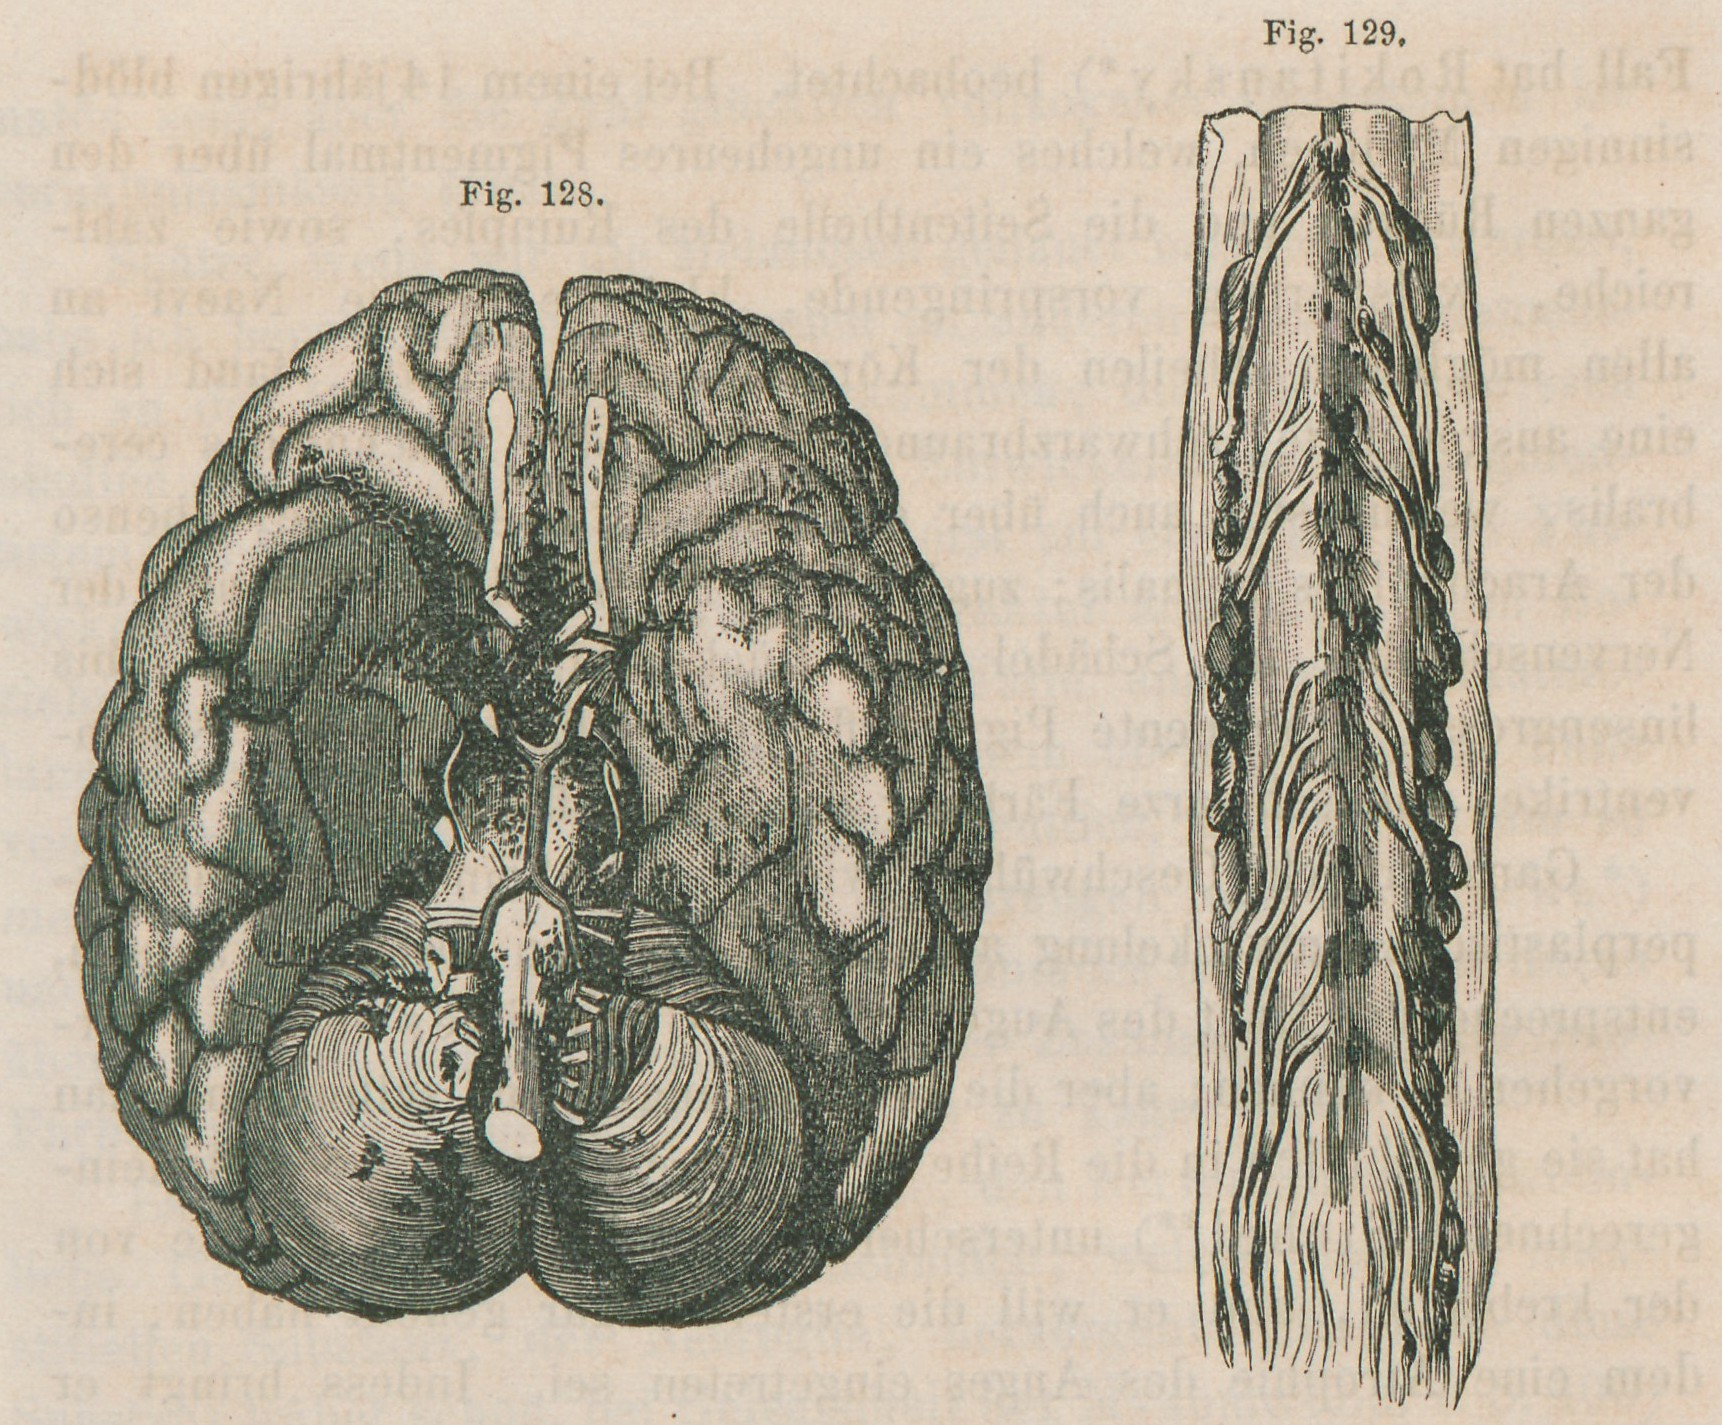
\includegraphics[width=.95\linewidth]{Figures/intro/drawingMelaMeta}
\caption[Drawing of central nervous system metastasis]{Drawing of central nervous system metastasis from page 121, Volume 2 of ``Die krankhaften Geschw\"ulste`` \protect\textcite{Virchow1863}; translated original caption: Fig. 128: Multiple melanoma of the Pia mater basilaris, most pronounced around the Medulla oblongata, the Pons, the Fossa Sylvii, Fissura longit (sample No. 256a from 1858); Fig. 129: Lower end of spinal cord of Fig. 128 with multiple melanoma of the soft skin with node like growths at the nerve roots (sample No. 256b from 1858)}\label{fig:drawing}
\end{figure}

While the search for possible cancer-causing substances started to gain more and more interest, only one real cause was thought to be found in the ore of the central European mountains, where miners would have a higher prevalence of lung cancers. Nevertheless, this was later found to be caused by radioactive material and not by the inhaled dust of minerals as expected. Similar\add{ly}, many parasites and bacteria were found as potential causes of cancer, but none of the findings could produce proof.

While all these steps were getting closer together in time up until the beginning of the 20$^{th}$ century, they were still fairly minor in contrast to the high speed of discoveries that the last hundred years brought with \change{it}{them}. While technically, Willhelm R\"ontgen discovered the X-rays just before the change of the century \cite{Roentgen1898}, its impact on the human body and cancer was only clear a few years into the last century \cite{Frieben1902,Scholtz1902}. However, similar to how X-rays can cause cancers, researchers also \add{quickly} found \remove{quickly} that \change{it}{they} can also treat cancer; thus the field of radiotherapy was created. \change{This}{Radiotherapy} then was the first \change{major}{significant} change in cancer treatment for around five thousand years, which also could treat inoperable cancers.

The \change{next}{following} invention \remove{that} I want to highlight within the vast amount of advances made in the advent of the 20$^{th}$ century, is the cutting needle aspiration syringe, which allowed a non-traumatic biopsy of internal organs for microscopy study. This biopsy method made it possible \add{not} to \remove{not} have exploratory surgery and \remove{instead} allowed improved diagnosis and planning of necessary surgery.

The next major step in the treatment of cancers comes in the form of chemotherapy when \textcite{Ehrlich1909} published his work ``Beitr\"age zur experimentellen Pathologie und Chemotherapy``, where he injected animals with different toxins in order to destroy cancer cells. Although, it still took another 30 years until after the second world war when it was discovered, that a chemical designed for warfare also had a potent anti-tumour effect.

In the meantime, the first long-term tissue cultures of animal cancer cell lines were established and further insights like the Warburg effect \cite{Warburg1928} \add{were} found, which showed that cancer cells use glucose at a higher rate than healthy cells. This effect ultimately led to the discovery of the positron emission tomography (PET) scan, which allowed a significantly more granular diagnosis and localisation of cancerous lesions than before.

With the success of growing human cell lines in vitro, the USA embarked on a massive experiment to test any potential source of chemical carcinogenesis. However, at the same time, multiple viruses were identified to cause cancers in the 1950s, when electron microscopy was invented \cite{Claude1947}.

Only a few more years later, the biggest advance in the understanding of biology was made when the structure of DNA was discovered \cite{Watson1953} (\autoref{intro-sec:DNA}), \change{and}{which} subsequently lead to numerous new experiments and breakthroughs. \add{For example,} when studying how viruses \change{are able to}{can} reverse transcribe their RNA and insert a new gene into a healthy cell, which then transformed into a cancer cell, the term ``oncogene`` was coined \cite{Huebner1969,Baltimore1970,Temin1970} and the foundation for the understanding of how genes influence the emergence of cancers was laid. This knowledge also lead to the understanding that heritable changes in the genome could predispose a person to cancer, which was previously hypothesised \cite{Li1969}. And while the discovery of DNA was a substantial boost for the understanding of cancer, the diagnostic capabilities increased at a similar speed, with urine tests for biomarkers of certain cancers as well as antigen detection.

\change{And}{Lastly} this is when we arrive at the ``current`` times when a few years ago, next-generation sequencing (NGS) (\autoref{intro-sec:sequencing}) was introduced and sped up data generation to improve our understanding of the genetic landscapes of different cancers and the subsequent development of genomic tests based on the molecular profile of certain cancers.
The completion of the ``Human Genome Project`` (\autoref{intro-sec:sequencing}) allowed the accurate resolution of common mutations in cancers, and consortiums coordinated large efforts to build databases of all somatic variations like TCGA, ICGC and PCAWG \cite{IPCAWGC2020}.

\add{These efforts then allowed the field to classify cancers depending on their tumour mutational burden (TMB), as not all cancer types are mutationally driven. While a typical akute myloid leukemia (AML) patient might only present with less than five somatic variants, a melanoma patient's cancer can show thousands of somatic mutations. In addition to somatic variations in cancer, there are many germline variants which cause a predisposition to cancer, like \textit{BRCA1/2}}\cite{Mersch2014}\add{ or \textit{TP53}}\cite{Li1969}\add{ and while some cancers have hundreds of thousands of somatic variants, they will also have millions of germline variants}\cite{Tiao2020}\add{. The combinatory space spanned by the somatic and germline variants of the cancer means that no cancer patients is like another and is known as inter-patient heterogeneity.}

However, with the genetic classification and investigation of cancers, researchers observed genetic heterogeneity in addition to the already well-established inter-patient heterogeneity\cite{Swanton2012}. Not all cancer cells in a patient share the same genetic setup, and this allows the disease to adjust and adapt to treatments and ultimately causes resistance \cite{Burrell2014}. \add{While in some patients the genetic heterogeneity is already present before treatment and selective pressure on the subclonal structure of the disease changes the composition}{\cite{Jakobsen2018}\add{, in others the resistance to treatment is likely non-genetic, but over time the cancer acquires a genetic resistance mechanism}\cite{Oxnard2018}\add{.}

Genetic pathology nevertheless enabled the identification of cancer vulnerabilities that then allowed the application of highly specific drugs, like tyrosine kinase inhibitors (TKI)s, which are tailored to target a specific alteration in the genome of a cancer cell, and genetically engineered antibodies \change{which}{that} can \remove{be} hone in on the cancer. 

While the therapeutic world is quickly evolving, many of the questions from previous times are still the same. We still \change{don't}{do not} know how and when the heterogeneity in cancers occurs. We \change{just}{,however,} know it is a major source of resistance to treatment. In \change{the majority of}{most} cancer types, we \remove{also} still do not have an answer to the ``cell of origin`` question that has been asked for so long.


So instead of trying to answer these questions directly, there has been an effort to define fundamental features of malignancies very similar to the early pathology descriptions.  The original characteristics comprise 
\begin{enumerate*}
	\item Sustaining proliferative signalling
	\item Evading growth suppressors
	\item Activating invasion and metastasis
	\item Enabling replicative immortality
	\item Inducing angiogenesis
	\item Resisting cell death
\end{enumerate*} (\autoref{fig:oldhallmarks}). 


\begin{figure}[hbtp]
\centering
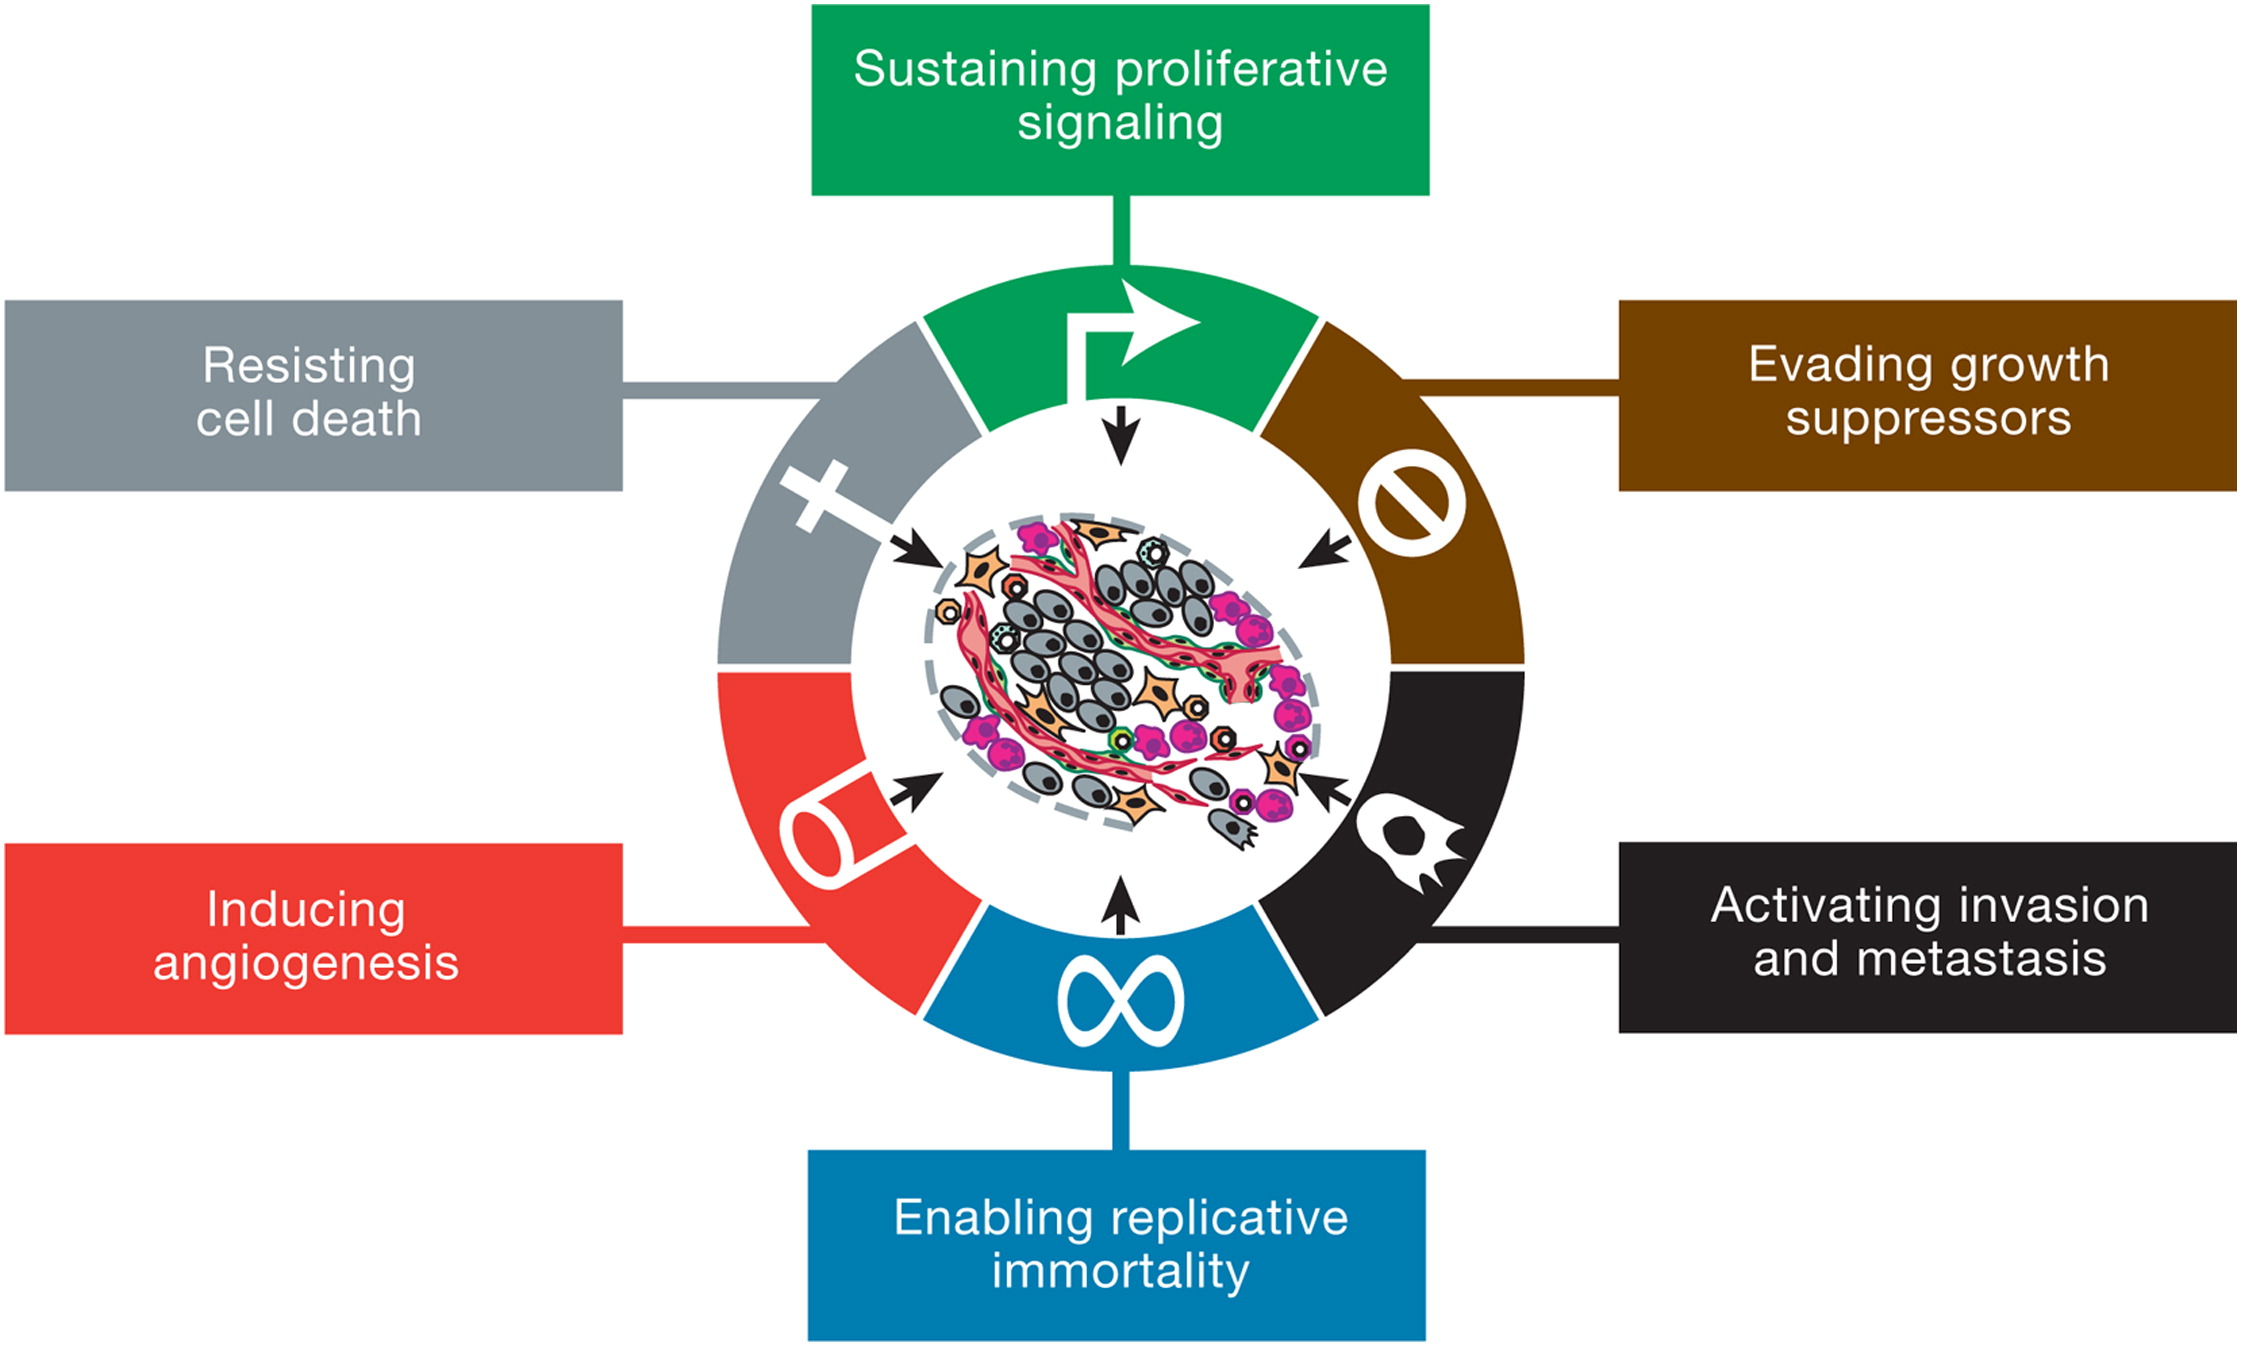
\includegraphics[width=.9\linewidth]{Figures/intro/oldHallmarksCancer.jpg}
\caption[Original hallmarks of cancer]{Acquired capabilities of cancer; Functional capabilities acquired by most cancers during their development; Figure adapted from \protect\textcite{Hanahan2000}}\label{fig:oldhallmarks}
\end{figure}



These hallmarks were for a while considered the core of tumour development, and the authors themselves hypothesised, that these core mechanics allow us to condense the complexity that cancer displays, both in the clinic and in labs, with a small set of rules, which all cancers have to obey \cite{Hanahan2000}. In their exact words: ``We foresee cancer research developing into a logical science, where the complexities of the disease, described in the laboratory and clinic, will become understandable in terms of a few underlying principles``

However, with 11 years of additional research into the topic, more hallmarks have been found, and \change{the original list was revised by the authors}{the authors revised the original list} to contain additional characteristics, namely 
\begin{enumerate*}
\item Avoiding immune destruction
\item Tumour-promoting inflammation
\item Genome instability and mutation
\item Deregulating cellular energetics
\end{enumerate*} \cite{Hanahan2011}. And even then, a few years later, even more hallmarks, e.g. metabolic rewiring, are now considered a part of the characteristics of cancer \cite{Fouad2017}.


\begin{figure}[hbp]
\centering
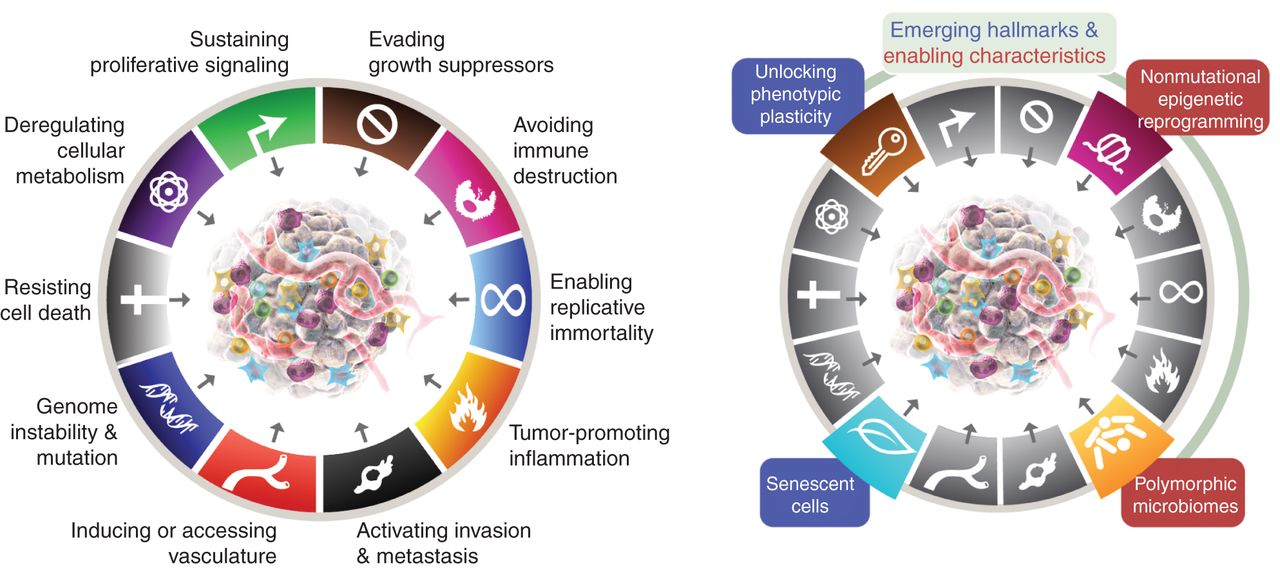
\includegraphics[width=.9\linewidth]{Figures/intro/NewestHallmarksOfCancer.jpg}
\caption[Newest hallmarks of cancer]{Emerging hallmarks and enabling characteristics of cancer; updated version of the hallmarks figure (\autoref{fig:oldhallmarks}, \cite{Hanahan2000}); Figure adapted from \protect\textcite{Hanahan2022}; Left, the Hallmarks of Cancer currently embody eight hallmark capabilities and two enabling characteristics. In addition to the six acquired capabilities -- Hallmarks of Cancer -- proposed in 2000 (\autoref{fig:oldhallmarks}), the two provisional “emerging hallmarks” introduced in 2011 \cite{Hanahan2011} --cellular energetics (now described more broadly as “reprogramming cellular metabolism”) and “avoiding immune destruction” -- have been sufficiently validated to be considered part of the core set. Given the growing appreciation that tumors can become sufficiently vascularized either by switching on angiogenesis or by co-opting normal tissue vessels \cite{Kuczynski2019}, this hallmark is also more broadly defined as the capability to induce or otherwise access, principally by invasion and metastasis, vasculature that supports tumor growth. The 2011 sequel further incorporated “tumor-promoting inflammation” as a second enabling characteristic, complementing overarching “genome instability and mutation,” which together were fundamentally involved in activating the eight hallmark (functional) capabilities necessary for tumor growth and progression. Right, this review incorporates additional proposed emerging hallmarks and enabling characteristics involving “unlocking phenotypic plasticity,” “nonmutational epigenetic reprogramming,” “polymorphic microbiomes,” and “senescent cells.”}\label{fig:newesthallmarks}
\end{figure}

And even during the time of my PhD, further research revealed additional hallmarks, which got characterised by \textcite{Hanahan2022}. The newest version adds another two characteristics and hallmarks, specifically:
\begin{enumerate*}
\item unlocking phenotypic plasticity 
\item nonmutational epigenetic reprogramming
\item polymorphic microbiomes
\item senescent cells
\end{enumerate*} 
(see \autoref{fig:newesthallmarks}).

The evolution of these hallmarks shows that even though much time and effort was invested in cancer research for multiple centuries, there is still no unifying definition and treatment for cancer. \add{Additionally,} the vast heterogeneity not only between cancer types but also between patients makes it very hard to study. More so, even within \add{a} patient there is \add{a} third type of heterogeneity, which is the \change{main}{leading} cause of treatment resistance and relapse \cite{DagogoJack2017}. Spatial heterogeneity refers to the non-uniform distribution of cancer subclones within different sites of disease. Even when the primary \change{site of disease}{disease site} is known, metastatic sites may show a very different genetic landscape. In contrast, temporal heterogeneity describes the changes \change{of}{in} a lesion over time. These changes can be caused by cancer progression or treatment (\autoref{fig:heterogeneities}). These two concepts, however, are not mutually exclusive, but can occur at the same time.

\begin{figure}[ht]
\centering
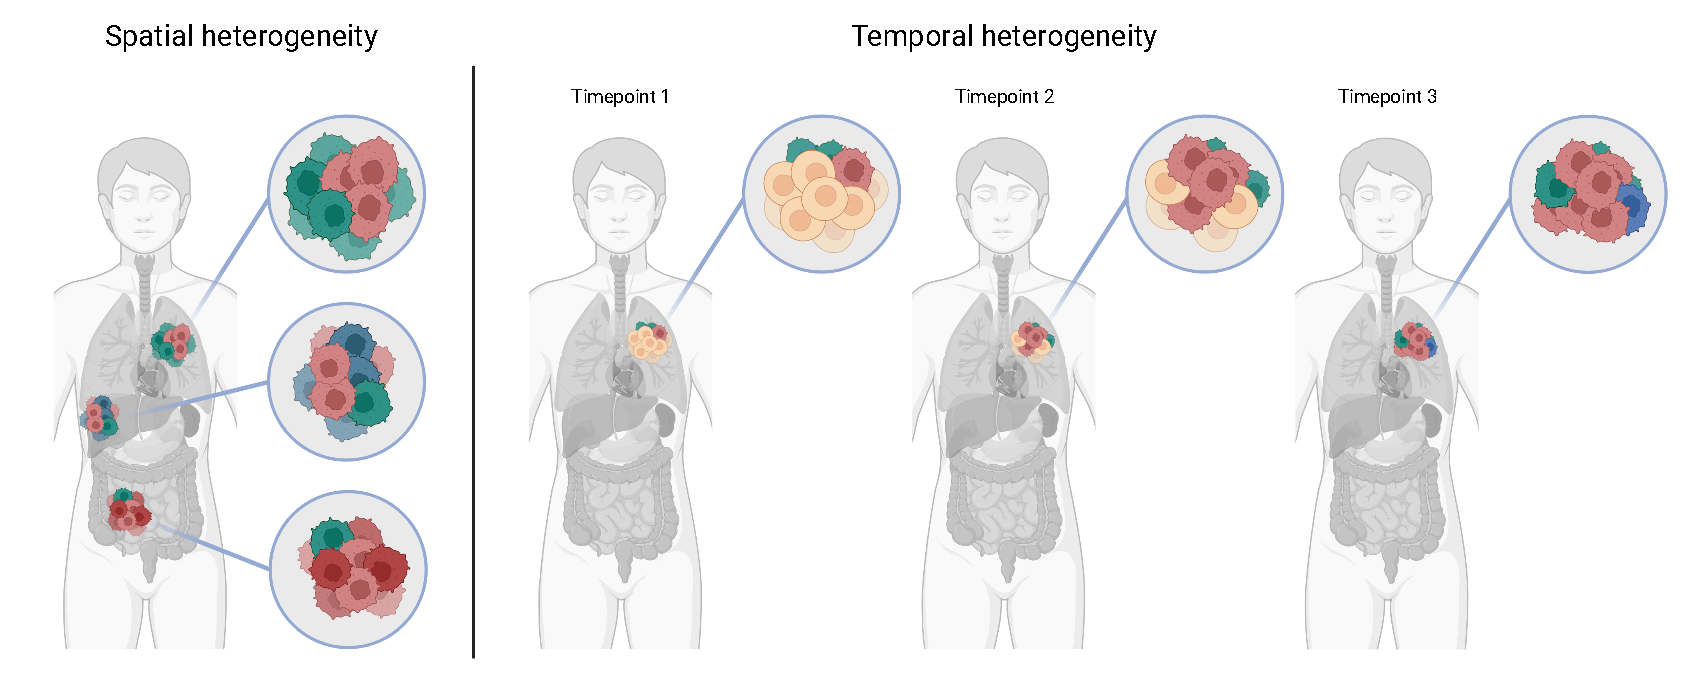
\includegraphics[width=.95\linewidth]{Figures/intro/heterogeneities.pdf}
\caption[Intra patient heterogeneities in cancer]{Types of intra patient heterogeneity in cancer: Spatial uneven distribution of subclones in different sites (left); Temporal heterogeneity with regards to genetic landscape within one site, either through progression of tumour or adaptation to treatment; Cells with rough membrane depict cancer cells, smooth membrane are normal cell. Colours show subclonal differences in the cancer. Figure adapted from \protect\textcite{DagogoJack2017}}\label{fig:heterogeneities}
\end{figure}


And while we know that this diversity exists and efforts have been made to measure and classify them \cite{Noorbakhsh2018}, there is still a lack of methods to directly analyse this heterogeneity and utilise this information to guide clinical approaches directly.

